\chapter{As vantagens de governar: o impacto da vitória nas eleições para prefeito na capacidade do partido em atrair apoiadores}
\label{cap:mecanismos}

Nos capítulos anteriores exploramos a relação entre prefeitos e candidatos aos demais níveis de governo com a finalidade de observar se os resultados das eleições municipais afetam tanto o desempenho eleitoral futuro de um partido quanto a decisão dos membros deste partido no Congresso Nacional. Uma das conclusões centrais é que prefeitos produzem vantagens eleitorais para os candidatos de seu partido nas eleições estaduais e nacionais, ainda que a existência destes efeitos dependa de algumas circunstâncias da competição local e varie entre anos.

O empreendimento do Capítulo~\ref{cap:eleicoes} se assemelha bastante ao de um conjunto de trabalhos preocupados em estimar a vantagem eleitoral do incumbente, que pode ser compreendida como a expectativa de que os candidatos ou partidos concorrendo a mais um mandato tenham chances sistematicamente maiores de serem eleitos em comparação a seus opontentes. Tanto dentro quanto fora do Brasil se produziu evidências contra e a favor à existência da vantagem do incumbente. Contudo, seja nestes trabalhos, seja no primeiro capítulo desta tese, raramente se questiona como vencer as eleições produz vantagens eleitorais para o partido. Em outras palavras, a literatura se concentrou na existência dos efeitos e não nos mecanismos que o produzem.

O objetivo do capítulo final desta tese é explorar alguns dos possíveis mecanismos pelos quais o partido consegue produzir vantagens eleitorais ao vencer uma disputa para um cargo majoritário. É possível pensar em vários mecanismos. Por exemplo, pode ser que prefeitos sejam um ponto focal cujo indicativo de apoio a um candidato (nas eleições nacionais/estaduais ou mesmo na disputa seguinte para prefeito) aumente as chances de vitória deste candidato. Pode ser também que prefeitos sejam capazes de ampliar gastos públicos na véspera da eleição para melhorar a imagem do partido. Ou ainda, é possível que prefeitos contratem novos servidores para a prefeitura na expectativa de atrair novos aliados e apoiadores no município. A lista de hipóteses ou conjecturas é grande e há trabalhos que sugerem a existência de vários destes mecanismos.

Neste capítulo, aproveitando do desenho de pesquisa já utilizado nos capítulos anteriores, estimo o efeito da vitória nas eleições municipais em três variáveis que potencialmente afetam os resultados das eleições municipais seguintes e que podem revelar alguns dos mecanismos pelos quais o partido é capaz de produzir vantagens eleitorais após uma vitória. São elas: 1 - o número de membros filiados ao partido; 2 - as receitas de campanha do partido para as eleições proporcionais no município; e 3 - o número de partidos aliados na competição pelo Executivo municipal. 

As hipóteses que dão origem a estes testes são bastante diretas. A expectativa é que o prefeito vencedor seja capaz de atrair mais membros para seu partido -- seja pela capacidade de contratar correligionários para a prefeitura, de fortaceler os diretórios partidários ou simplesmente de se apresentar como organização capaz de influenciar políticas municipais. Da mesma forma, espera-se que um partido vitorioso seja capaz de arrecadar mais recursos para suas campanhas futuras para outros cargos, como, por exemplo, nas disputas para vereador no município. Além do prefeito ter a possibilidade de contratar serviços e comprar insumos de empresas no município que no futuro podem contribuir para a campanha do partido, o simples fato de vencer as eleições em um ano aumenta as chances do partido vir a apresentar candidatos competitivos nas eleições seguintes e, portanto, de atrair doadores para sua campanha. É bastante razoável que um partido vitorioso consiga manter doadores entre eleições e também de atrair novas contribuições.

Por fim, se é verdade que também nos municípios o chefe do Executivo é capaz de atrair os demais partidos para construção de coalizões de governo, e que as coligações eleitorais refletem tais coalizões, é de se esperar que partidos vitoriosos sejam capazes de construir coalizões municipais maiores ou, pelo menos, contem com o apoio de um percentual maior de vereadores de outras siglas.

As perguntas que orientam os três testes podem ser resumidas em uma única: o partido vitorioso nas eleições municipais é capaz de atrair novos apoiadores, sejam eles novos membros, doadores de campanhas ou políticos de outros partidos interessados na administração municipal? Nas próximas seções discuto com mais detalhes cada um dos problemas em separado.

Nos capítulos anteriores o foco da análise era a relação entre prefeitos com membros e candidatos do partido nos demais níveis de governo. Note-se que neste capítulo os atores estaduais e nacionais estão fora da análise e me concentro apenas nas consequências da vitória para a construção de capacidade competitiva do partido dentro do próprio município. As razões para tal escolha derivam dos limites para se medir ou coletar dados sobre os fenômenos estudados, como será explicado adiante. O vínculo com os demais esforços de pesquisa provém da suspeita de que as vantagens conquistadas no município servem também ao partido nas disputas políticos para outros níveis de governo.

Diferentemente das etapas anteriores da pesquisa, os resultados deste capítulo apontam para a inexistência dos mecanismos testados. Não há evidências de que vencer as eleições para prefeito afeta o número de filiados do partido, as receitas futuras do partido nas campanhas para vereador ou o tamanho das coalizões eleitorais emcabeçadas pelo partido no município. Há evidências frágeis do efeito do tratamento na arrecadação de campanha do partido nas eleições para vereador. Este resultado, porém, tem baixa validade e há um possível viés na sua estimação. O único resultado positivo expressivo apresentado no capítulo aponta para a existência de efeito do tratamento - governar o município - no número de filiados ao partido na metade do mandato do prefeito.

Este capítulo está organizado de maneira um pouco diferente dos demais. Dedico cada seção do capítulo à investigação de cada uma das três hipótese. Desta forma, percorro rapidamente o caminho que leva da construção do problema à apresentação dos dados e discussão dos resultados para cada mecanismo. A próxima seção revê os fundamentos do desenho de regressão descontínua adotado na tese e sua aplicação na investigação das hipóteses deste capítulo. As seções seguintes tratam da análise do impacto da vitória para prefeito no número de filiados do partido, nas receitas de campanha do partido e no tamanho das coligações eleitorais, nesta ordem. Ao final, discuto brevemente os resultados.

\section{A mecânica da regressão descontínua e a construção de vantagens eleitorais}

A estratégia de investigação empírica deste capítulo é a mesma dos anteriores. A votação de um partido $p$ para uma eleição para prefeito no ano $t$ no município $m$ ($V_{p,m,t}$ ou $V_{i}$, sendo $i$ uma combinação de $p$, $t$ e $m$) pode ser descrita em termos de uma função densidade de probabilidade condicional às diversas características do partido no município, representados por $A_{i}$, e assumidos aqui como não observáveis, e por um termo aleatório $\epsilon_{i}$. 

Nos municípios brasileiros com menos de 200 mil eleitores aptos os candidatos disputam uma eleição majoritária de apenas um turno para a prefeitura e vence as eleições o candidato que obtiver o maior número de votos ($V_{i}$). Governará o partido ($d_{i}=1$) que tiver maior $V_{i}$ e margem de votos positiva em relação ao partido oponente mais bem votado ($\tau_{i}=\Delta>0$). Cada partido tem uma probabilidade diferente de governar ou não o município e esta probabilidade depende de $A_{i}$.

O objetivo é estimar o efeito do tratamento $d_{i}$ em $Y_{i}$, variável resposta que também é função de $A_{i}$ e que pode ser descrita da mesma forma que $V_{i}$. Este é o caso das variáveis dependentes deste capítulo. Número de filiados, receitas de campanha e tamanho das coalizões eleitorais são atributos do partido no município e variam no tempo. O número de filiados pode ser medido em qualquer momento entre eleições municipais. Receitas de campanha e tamanho das coalizões podem ser observados apenas em anos eleitorais.

$d_{i}$ e $Y_{i}$ são função dos mesmos conjuntos de variáveis e a condição de independência $Y_{i} \perp d_{i}$ não é válida. Contudo,  quando o módulo margem de vitória tende a zero temos que a probabilidade de um partido, em um município e em uma eleição específica é independente do fatores não observáveis ($A_{i}$) que determinam $\tau_{i}$. Logo: 

\[
\lim_{\Delta \to 0} E[d_{i}|\tau_{i}=-\Delta]=\lim_{\Delta \to 0} E[d_{i}|\tau_{i}=+\Delta]
\]

A consequência do tratamento ser quase aleatório é que podemos estimar o efeito $\rho$ do tratmento $d_{i}$ em $Y_{i}$ da seguinte maneira:

\[\rho =\lim_{\Delta \to 0} E[E[Y_{i}|d_{i}=1]|\tau_{i}=+\Delta] - \lim_{\Delta \to 0} E[E[Y_{i}|d_{i}=0]|\tau_{i}=-\Delta]\]
\[=\lim_{\Delta \to 0} E[Y_{1,i}|\tau_{i}=+\Delta] - \lim_{\Delta \to 0} E[Y_{0,i}|\tau_{i}=-\Delta]\]
\[=\lim_{\Delta \to 0} (E[Y_{1,i}|\tau_{i}=+\Delta] - E[Y_{0,i}|\tau_{i}=-\Delta])\]

Novamente, apresento os resultados do efeito causal, $\rho$, em função de $\Delta$ (para evitar a escolha de uma margem de vitória arbitrária) e de três maneiras diferentes: como diferença de médias entre os grupos de tratamento, como descontinuidade em um função linear de $Y_{i}$ por $\tau_{i}$ e como descontinuidade em um função polinomial de terceiro grau de $Y_{i}$ por $\tau_{i}$.

A interpretação da análise é semelhante à dos capítulos anteriores. Quando comparamos quase vencedores e quase perdedores, podemos observar diferenças quanto à capacidade do partido em atrair novos apoiadores, sejam eles novos membros filiados ao partido, apoiadores de campanha ou partidos aliados e seus respectivos vereadores? Se sim, então há evidências de que o partido vencedor no município consegue melhorar seu desempenho futuro por meio da atração de novos apoios. Se não, então atrair novos apoios não é um mecanismo relevante para explicar como os partidos políticos vitoriosos produzem obtêm vantagens eleitorais em relação a seus adversários.

\section{Prefeitos, campanhas e organização partidária: o efeito da vitória eleitoral no número de filiados ao partido}

Um dos aspectos críticos da democracia brasileira frequentemente apontado na literatura é o baixo grau de identificação dos eleitores com os partidos políticos. A filiação aos partidos reflete diretamente esta face do sistema político nacional: em 2010 o Brasil tinha aproximadamente 130 milhões de eleitores aptos e cerca de 14 milhões de pessoas filiadas a partidos políticos, ou seja, pouco mais de 10\% do total de pessoas registradas para votar. Certamente este número é maior do que o total de pessoas que efetivamente se engaja na política partidária, posto que o cadastro de filiados do TSE contém várias falhas de registro e a desfiliação não costuma ser algo recorrente entre membros que não têm pretensões eleitorais. Mais ainda, este valor está distribuído entre todos os partidos. O PMDB, partido com o maior número de filiados no país, conta com 1,7\% do total de eleitores filiados no país. O primeiro gráfico da Figura~\ref{fig:c3fil1} apresenta o número de filiados por partido.

Os trabalhos sobre filiação partidária e voto no Brasil normalmente utilizam dados de survey. Praticamente não há evidências sobre o efeito da filiação partidária no desempenho eleitoral e, tal como a presente pesquisa, do resultado eleitoral sobre a capacidade dos partidos atraírem novos membros. É possível conjecturar algumas razões para tal lacuna. A primeira é a qualidade dos dados sobre filiação partidária. Além dos problemas de registro e manutenção da filiação de membros inativos já mencionados, as listas de filiados dos partidos eram, até a pouco tempo atrás, raramente disponibilizadas a pesquisadores.

A segunda razão possível é que as teorias de mobilização, bastante importantes nos EUA e em países em que o voto não é compulsório, têm pouca aderência ao contexto brasileiro. Membros do partido são peças chave para levar eleitores para as urnas, mas talvez não tão importantes para influenciar a escolha do voto dos eleitores brasileiros. Sobretudo no caso das campanhas para cargos majoritários, com destaque para presidente, governador, senador e prefeitos de capitais, a comunicação em rádio, TV, internet e jornais têm mais relevância e consome mais recursos do que a persuasão por parte dos membros do partido do candidato. É bastante mais provável que o papel de correligionários em campanha seja mais importante nas eleições proporcionais ou em municípios menores.

Finalmente, os partidos brasileiros variam quanto à forma e grau de organização partidária. Inclusive, é possível notar diferenças dentro de um mesmo partido entre diferentes estados. Há partidos que contam com diretórios espalhados em vários municípios, enquanto outros têm apenas comitês provisórios ou têm abrangência territorial reduzida. Assim, ou a maioria dos partidos não têm capacidade para se espalhar pelo país todo, ou a construção de uma rede de diretórios, comitês e filiados não é um elemento crucial para a vitória nas eleições. Novamente, o pressuposto impacto reduzido da militância de membros do partido no resultado eleitoral pode ser uma explicação para a carência de trabalhos na literatura brasileira sobre o efeito dos filiados do partido no resultado das eleições e também de trabalhos sobre o problema reverso, ou seja, do efeito bom desempenho eleitoral no número de membros de uma organização.

Esta seção tem o objetivo de examinar se os partidos vitoriosos nas eleições municipais são capazes de atrair novos filiados. A pergunta poderia ser ampliada: há efeito do partido ter um bom desempenho eleitoral na capacidade do partido consolidar raízes no eleitorado? É possível imaginar algumas das razões pelas quais um partido poderia atrair novos eleitores após vencer as eleições, ainda que não seja possível testá-las. Em primeiro lugar, o partido vitorioso tem a prerrogativa de indicar pessoas para a nova administração municipal. Em segundo, pessoas ligadas ao partido tem maiores chances de influenciar o processo decisório de políticas públicas. A possibilidade de participar, seja da administração municipal, seja das decisões públicas, é uma vantagem relevante para o partido vitorioso.

Tal como no primeiro capítulo, é fundamental compreender que a hipótese desta seção é composta de duas partes. Para que haja efeito do tratamento no número de filiados do partido, é preciso que as condições seguintes sejam simultaneamente satisfeitas: 1- a vitória para prefeito deve aumentar o interesse das pessoas pelo partido; e 2- este interesse deve ser transformado em novas filiações aos diretórios e comitês locais do partido. A ausência de efeito do tratamento signifca que pelo menos uma das duas condições acima não foi satisfeita.

A razão pelo qual um desenho de regressão descontínua serve aos propósitos deste capítulo é bastante simples. A expectativa é que o partido tenha um desempenho eleitoral na eleição municipal bom em municípios onde há maior suporte no eleitorado e consequentemente, nos quais o partido tem um número relativamente maior de filiados. Dessa forma, observar diretamente a correlação entre vencer as eleições e o crescimento no número de filiações do partido é analiticamente incorreto. 

Antes de avançar na análise do efeito da vitória, convém debater rapidamente os dados utilizados, a operacionalização da pesquisa e testar a validade da adoção de um desenho de regressão descontínua para o problema investigado nesta seção.

\subsection{Operacionalização da pesquisa, dados utilizados e validade do desenho de regressão descontínua}

Os dados utilizados nesta seção provém do próprio Tribunal Superior Eleitoral. A partir da listagem de filiações foi possível construir para cada ano o total de filiados por partido e por município. Os dados de filiados têm registros bastante antigos, inclusive alguns do final da década de 70. Entretanto, os dados são pouco confiáveis qualquer período anterior à segunda metade dos anos 1990. Pelo período em que os dados foram coletados, os registros para 2011 são incompletos. Não há dados partir do ano 2012 neste trabalho. A data de referência utilizada para medir quantos filiados havia no partido e no município por ano foi primeiro de julho, ou seja, sempre antes das eleições e antes do início das campanhas eleitorais (nos anos em que há eleições).

O número absoluto de filiados que um partido tem em um município é certamente proporcional ao eleitorado local. Por esta razão, é preciso medir $Y_{i}$ com um denominador que torne os municípios comparáveis entre si. Para esta seção, utilizo duas maneiras diferentes de medir $Y_{i}$. A primeira delas é simplesmente a variação percentual do total de filiados nos quatro anos após a eleição municipal $t$, na qual os grupos de tratamento e controle foram definidos. A medida de variação é bastante simples e adequada ao problema. Contudo, em situações em que o município tem poucos eleitores, a entrada ou saída de um novo membro para o partido representa uma variação muito grande. Por esta razão utilizo também uma segunda medida: o total de filiados quatro anos após $t$, ano da eleição municipal, sobre o total de eleitores aptos no município.

Ao utilizar informação de filiados quatro anos após as eleições municipais, é necessário excluir da análise as observações das eleições municipais de 2008, posto que os dados de filiação utilizados não permitem ir além de 2010. Por esta razão, repito o procedimento de análise substituindo em ambas medidas de $Y_{i}$ o número de filiados quatro anos após $t$ pelo número de filiados dois anos após $t$. Medir a filiação dois anos após a eleição municipal também tem um sentido prático importante, pois é exatamente o momento em que ocorrem as eleições estaduais e nacionais e no qual se espera que os membros do partido estejam mobilizados e engajados nas campanhas. Além disso, a grande maioria dos prefeitos que trocam de partido ao longo do mandato o fazem entre julho e setembro do terceiro ano no governo municipal. Dessa forma, a medida de $Y_{i}$ para os dois primeiros anos sofre menos com migração de prefeitos do que a medida de $Y_{i}$ para os quatro anos de mandato.

\begin{figure}[htp]
	\centering
	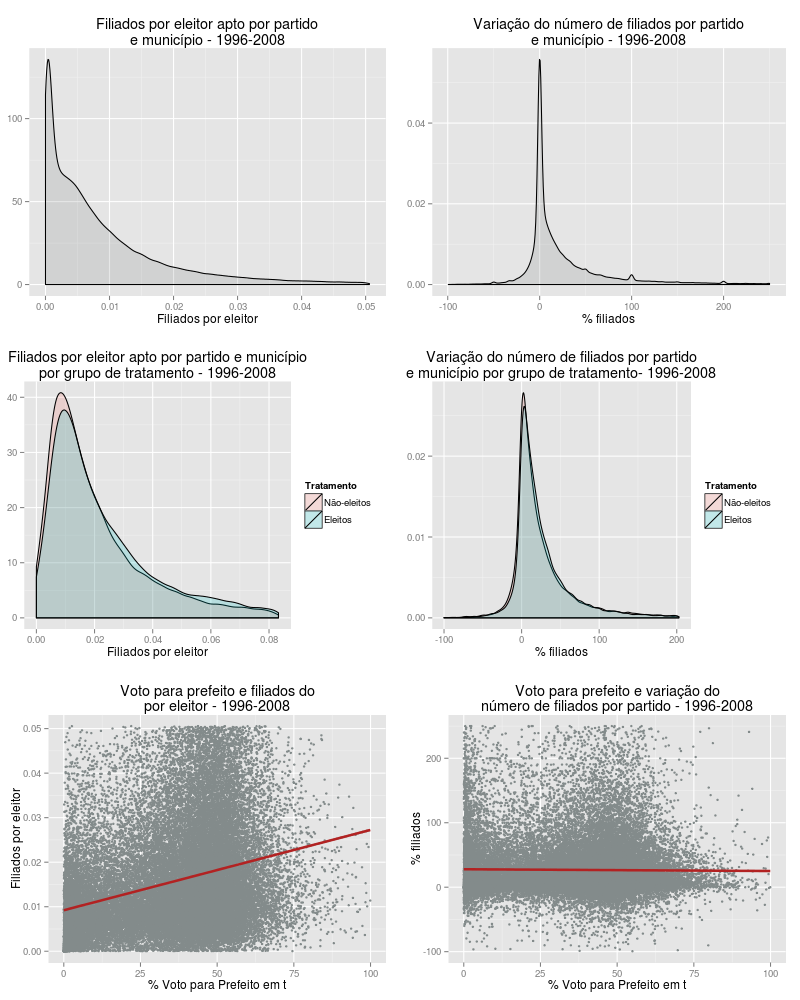
\includegraphics[scale=0.5]{c3fil1.png}
	\caption{Distribuição do número de filiados (por eleitor ou como variação durante o mandato) de 1996 a 2008: 1 - para todos os partidos em todos os municípios; 2 - para os partidos incluídos na análise e separado por grupos de tratamento; e 3 - por voto para prefeito na eleição anterior.}
	\label{fig:c3fil1}
\end{figure}

Convém agora examinarmos a distribuição das variáveis utilizadas no capítulo. A Figura~\ref{fig:c3fil1} apresenta, para cada uma das medidas adotadas, a distribuição do número de filiados para todos os partidos brasieliros por município, a distribuição do número de filiados para todos os partidos brasileiros por município apenas para as observações que compõem a análise e separados por grupo de tratamento e, finalmente, a distribuição de $Y_{i}$ pelo voto do partido nas eleições para prefeito. Este último gráfico contém também uma reta de regressão linear que representa a relação entre as duas variáveis. Os gráficos à esquerda representam a variável $Y_{i}$ medida como número de filiados por eleitor no município. Os gráficos à direita representam $Y_{i}$ medida como a variação do total de filiados do partido no município em 4 anos. 

Há algumas observações importantes sobre a distribuição de $Y_{i}$. Quando a medida adotada é a proporção de filiados por eleitor quatro anos após a eleição, vemos que a distribuição é bastante assimétrica para o universo e para os dados que compõem a análise. Há poucas diferenças entre os grupos de tratamento, ainda que seja possível observar mais unidades não tratadas para os menores valores e mais unidades tratadas para os maiores valores. Há uma clara correlação da variável com o voto para prefeito e, consequentemente, com a margem de vitória.

Quando se observa $Y_{i}$ medida como variação ao longo do mandato, porém, não é possível notar nenhuma relação com a margem de vitória. A reta de regressão que descreve a distribuição conjunta dos dados é praticamente horizontal. Esta é uma importante pista de que $Y_{i}$ medida desta forma não está correlacionado com os fatores não observáveis ($A_{i}$)  que explicam a margem de vitória e, consequentemente, as chances de tratamento. A variação percentual no número de filiados por partido nos municípios para o universo está concentrada no zero. Para os dados da amostra a dispersão é um pouco maior e, novamente, as diferenças entre os grupos de tratamento são pequenas.

Repetindo o procedimento adotado anteriormente na tese, para verificar se a adoção de um desenho de regressão descontínua é adequada ao problema, testo se o tratamento explica variáveis $O_{i}$ que, por construção, não podem sofrer impacto do tratmento. Nesta seção, utilizo tanto a variação percentual no mandato anterior quanto o número de filiados por eleitor em julho do ano das eleições municipais em $t$. No primeiro caso, são incluídas somente as eleições municipais de 2000 e 2004 posto que os dados sobre filiação partidária para 1992 são de baixa qualidade e 2008 está, num primeiro momento, fora da análise. No segundo caso, o período testado inclui 1996 e mantém a exlusão de 2008. Os resultados são apresentados na Figura~\ref{fig:c3fil2}.

\begin{figure}[htp]
	\centering
	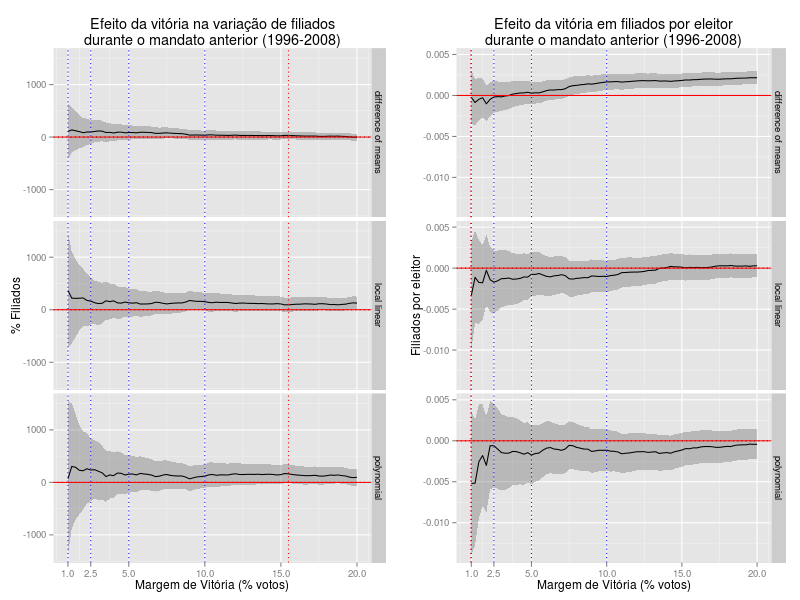
\includegraphics[scale=0.5]{c3fil2.png}
	\caption{Efeito do Tratamento no número de filiados do partido (na data da eleição por eleitor ou como variação no mandato anterior) por margem de vitórias nas eleições para prefeito (1996-2010).}
	\label{fig:c3fil2}
\end{figure}

Claramente, o tratamento não explica nenhuma das duas medidas de $O_{i}$, ou seja, não há nenhum efeito da vitória nas eleições municipais na quantidade de membros que o partido tem no passado. Mesmo quando a variável $O_{i}$ é representada pela proporção de filiados ao partido no eleitorado, variável que tem correlação positiva com a margem de vitória na eleição municípal, não temos nenhuma evidência de que haja desbalanceamento entre os grupos de tratamento. Este resultado torna seguro estimar o efeito do tratamento no futuro, propósito deste capítulo. Podemos também contar com as análise já produzidas para os demais capítulos, que apontam para a inexistência de efeito do tratamento em outras variáveis passadas, como o próprio voto para prefeito quatro anos antes da eleição em $t$, os votos nas eleições nacionais e estaduais dois anos antes de $t$, o voto para vereador em $t$ ou o total de emendas apresentadas pelos membros do partido nos anos anteriores à eleição municipal\footnote{O Capítulo~\ref{cap:financiamento} retoma o tema do desequiblíbrio entre os grupos de tratados e não tratados e apresenta problemas inicialmente não discutidos nesta seção. Como se observará adiante, há uma variável para a qual o desequilíbrio entre tratados e não tratados é mais sério: as receitas de campanha para prefeito. Sistematicamente, partidos vitoriosos arrecadaram mais do que partidos derrotados, mesmo quando são comparados apenas os casos nos quais a margem de vitória tende a zero. O Capítulo~\ref{cap:financiamento} trata apenas deste assunto e revê os resultados dos três primeiros capítulos à luz deste problema.}.

\subsection{O efeito da vitória nas eleições municipais sobre o número de filiados ao partido}

Partidos vitoriosos no município conseguem atrair novos apoiadores para o partido? Estes novos apoiadores tornam-se filiados ao partido? Este é o objeto de investigação desta seção. A suspeita é que o partido que conquista a prefeitura é capaz de aumentar o número de filiados no município e que este é um dos mecanismos pelos quais podemos observar efeitos da vitória para prefeito, por exemplo, nas eleições nacionais e estaduais.

A Figura~\ref{fig:c3fil3} apresenta os resultados para o período de 1996 a 2008. É importante lembrar que as eleições de 2008 estão excluídas em virtude da ausência de dados para filiados em 2012.

\begin{figure}[htp]
	\centering
	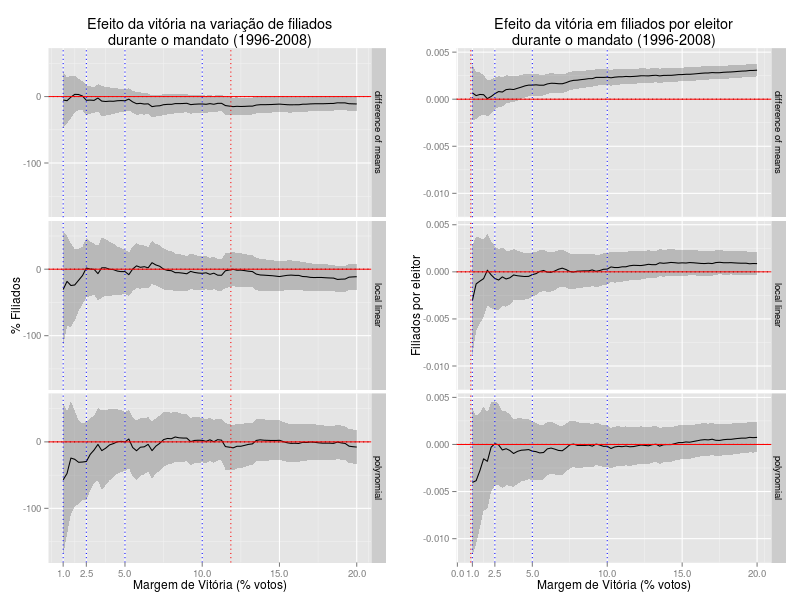
\includegraphics[scale=0.5]{c3fil3.png}
	\caption{Efeito do Tratamento no número de filiados do partido (ao final do mandato por eleitor ou como variação no mandato) por margem de vitórias nas eleições para prefeito (1996-2008).}
	\label{fig:c3fil3}
\end{figure}

Não há nenhuma evidência de que vencer as eleições municipais tem efeito no número de filiados do partido. O efeito do tratamento, $\rho$, é diferente de zero apenas quando estimado por diferença de médias e para margens de vitórias menores ou iguais ao ponto em que $\Delta \leq 5\%$. Porém, dado o exame de validade do desenho de pesquisa dos capítulos anteriores, sabemos que nesta circunstância o efeito estimado pode ser viesado. O resultado nulo independe da medida, ou seja, o vencer as eleições no município não tem efeito sobre o número de filiados por eleitor do partido no município ou sobre a taxa de variação do número de filiados por partido entre anos.

Há duas leituras possíveis deste resultado nulo. O primeiro deles é que vencer as eleições para prefeito não contribui para que o partido atraia novos apoiadores, ainda que, como vimos, o desempenho eleitoral do partido aumente. Se esta explicação for verdadeira, vencer as eleições para prefeito tem efeito na atração de novos eleitores mas não de filiados ao partido.

A segunda interpretação é que, mesmo atraindo novos apoiadores para o partido, estes não terminam por se filiar ao partido. Dito de outra forma, o partido consegue fazer com que mais pessoas participem de sua administração e de sua campanha, mas estas nosos apoiadores não optam por serem membros formais do partido.

Para poder incluir as eleições de 2008 na análise, repito o procedimento acima adotado, mas, em vez de utilizar o número de filiados nas eleições quatro anos após a eleição municipal, construo ambas as medidas de $Y_{i}$ a partir do total de filiados ao partido no município dois anos após a disputa pelo Executivo municipal. Os resultados são apresentados na Figura~\ref{fig:c3fil4}

\begin{figure}[htp]
	\centering
	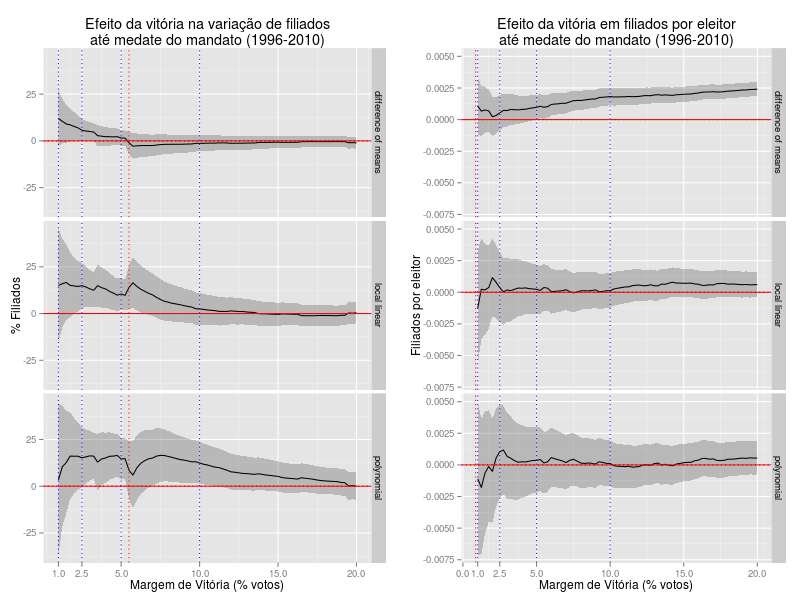
\includegraphics[scale=0.5]{c3fil4.png}
	\caption{Efeito do Tratamento no número de filiados do partido (na metade do mandato por eleitor ou como variação nos dois primeiros anos do mandato) por margem de vitórias nas eleições para prefeito (1996-2010).}
	\label{fig:c3fil4}
\end{figure}

Não há efeito algum do tratamento quando a variável dependente é o número de filiados ao partido no município por eleitor. Porém, quando observamos o efeito de vencer no município na taxa de variação do número de filiados nos dois primeiros anos do mandato do prefeito, encontramos um resultado positivo e diferente de zero, não importando, inclusive, a maneira com que o efeito do tratamento $\rho$ é estimado. Vencer as eleições faz com que o partido aumente em aproximadamente 14\% o número de membros registrados ao partido localmente - utilizando novamente a descontinuidade em uma regressão linear e módulo margem de vitória menor ou igual a 2.5\%.

Qual a razão do resultado divergir entre as duas medidas? A taxa de variação é bastante mais sensível ao tamanho do município do que o número de filiados por eleitor. É possível, pois, que a média da variação nos municípios menores -- que representam a maioria das observações -- seja maior do que nos municípios maiores. Qual a razão para o efeito nos dois primeiros anos ser relevante e o nos quatro anos de mandato não? Não há respostas claras a esta pergunta, mas uma possível razão é a migração entre partidos dos prefeitos. Usando dados dos prefeitos eleitos em 2000 e 2004, vemos que pouco menos de 5\% troca de partido até aś eleições estaduais/nacionais. Entretanto, quase um quinto terá migrado até o final do período legal para concorrer a eleições municipais por um novo partido, ou seja, na segunda metade do terceiro ano do mandato\footnote{fonte: elaboração própria a partir de dados de candidaturas e filiação partidária do TSE}. Se prefeitos que migram levam consigo membros filiados ao partido para uma nova agremiação, então é possível que o efeito de vencer as eleições no número de filiados seja mitigado pela migração partidária.

Temos, assim alguma evidência, ainda que frágil, de que pelo menos nos primeiros anos do mandato e provavelmente nos menores municípios vencer as eleições para prefeito contribui para aumentar o número de filiados ao partido. Considerando que as eleições para deputado federal e estadual ocorrem na metade do mandato do prefeito, não parece adequado descartar que a mobilização de novos membros do partido pelo prefeito seja um mecanismo importante, mesmo sob evidências empíricas frágeis.

A seguir, vamos examinar o efeito de vencer as eleições municipais sobre as receitas de campanha do partido nas eleições proporcionais no município subsequentes.

\section{Prefeitos, vereadores e campanhas: o efeito da vitória eleitoral nas receitas de campanha do partido para vereador}

Campanhas eleitorais vitoriosas em praticamente qualquer democracia têm um denominador comum: a capacidade de arrecadar recursos com empresas, membros do partido e eleitores individuais. A única exceção, talvez, sejam sistemas políticos nos quais o financiamento às campanhas provém na maior parte do próprio Estado. As campanhas mais caras não são necessariamente as campanhas vitoriosas, mas é raro encontrar em qualquer sistema político partidos verdadeiramente competitivos que não dependam da sua capacidade de arrecadar fundos para competir nas eleições. O Brasil claramente não é uma exceção. Para qualquer cargo que se observe, sempre há relação direta entre as receitas de campanha de um partido e seu desempenho eleitoral.

O desempenho eleitoral em uma eleição está correlacionado com a performance do partido na eleição anterior por serem ambos consequências de um conjunto comum de fatores não observáveis, aos quais anteriormente resumimos em $A_{i}$. Alguns desses fatores podem ser traduzidos como capital político, apoio no eleitorado, qualidade dos candidatos, etc. É bastante provável que algo semelhante ocorra com os recursos de campanha arrecadados por um partido. As receitas de um partido são, pelo menos em parte, resultado da expectativa de vitória e, portanto, desses mesmos fatores não observáveis. Campanhas caras produzem resultados eleitorais melhores e boa performance eleitoral produz expectativas maiores de vitória no futuro. Como separar, então, o efeito da vitórias nas eleições municipais nas receitas de campanha do desempenho eleitoral que produziu a vitória?

Responder à pergunta desta seção -- a vitória eleitoral tem impacto nas receitas de campanha futuras do partido? -- requer a adoção de uma estratégia investigativa que permita separar analiticamente o efeito dos fatores não observáveis que explicam simultaneamente o tratamento e a variável resposta.

É possível conjecturar diversas razões pelas quais a vitória nas eleições municipais produziria resultados positivos futuros na arrecadação de campanha do partido. Ao se mostrar vitorioso em uma disputa, o partido sinaliza a potenciais doadores de campanha chances altas de governar o município novamente. Entretanto, é bastante provável que o partido seja capaz de arrecadar mais para suas campanhas nas eleições seguintes pelo fato de que boa parte das doações para campanhas provém de pessoas jurídicas, muitas das quais têm interesse em decisões da prefeitura e em contratos para prestação de serviços ou fornecimento de produtos para o Estado. \citet{Samuels2008a} aponta que o objetivo de parlamentares ao particarem \emph{pork barrel} é conquistar financiadores de campanha que se beneficiam de contratos públicos e não necessariamente eleitores. Mesmo em se tratando de eleitores, é possível que o partido vencedor arrecade relativamente mais porque indivíduos interessados em nomeações para cargos em comissão decidam doar para as campanhas do partido. Testar tais conjecturas estão para além do escopo da tese e há análises empíricas na literatura que tratam de tais temas. Para a pesquisa apresentada nesta seção, é relevante apenas notar se o partido vitorioso obtém mais apoiadores dispostos a contribuir para as suas campanhas.

Infelizmente não há dados sobre receitas de campanhas nas disputas para os cargos eletivos nos estados e no governo federal identificáveis por município. O ideal seria observar se as receitas de campanha dos partidos para deputado federal, estadual, senador, governador e presidente são maiores nos municípios em que o partido governa em relação aos municípios nos quais o partido não governa. Como as contas das campanhas dos partidos para tais cargos são agregadas por estado -- ou mesmo nacionalmente, no caso da disputa para presidente -- atribuir uma doação de campanha a um partido em um município é praticamente impossível. Assim, opto por analisar apenas o impacto da vitória no município nas contas do partido nas eleições municipais seguintes. A suspeita é que se o partido -- ou prefeitos eleitos -- são capazes de conquistar doadores para o partido no município, também o serão quando buscarem doadores para as campanhas dos membros de seu partido que concorrem cargos em outros níveis de governo.

O problema central que decorre da utilização de dados de receita de campanhas municipais é que prefeitos podem ser competentes para conquistar apoiadores ao longo de seus mandatos para sua própria reeleição sem, no entanto, contribuirem para que o partido tenha caixas de campanha mais abastecidos. Há uma alternativa para contornar este problema: estimar o impacto da vitória nas contas do partido nas campanhas para vereador. Se prefeitos contribuem para que membros de seu partido concorrendo a cargos no Legislativo municipal tenham mais recursos para suas campanhas, é razoável supor que também contribuirão pelo menos para melhorar a arrecadação das campanhas de candidatos a deputados federais e estaduais do partido, sobretudo de parlamentares incumbentes. Vamos a seguir examinar os procedimentos de pesquisa, as variáveis utilizadas e a validade do desenho.

\subsection{Operacionalização da pesquisa, dados utilizados e validade do desenho de regressão descontínua}

O montante gasto pelos partidos nas campanhas municipais é, antes de mais nada, proporcional à população do município. Candidaturas a prefeituras em municípios grandes gastam consideravelmente mais do que candidaturas em cidades pequenas. Da mesma maneira, candidatos a vereador em grandes centros urbanos dispendem mais recursos do que competidores ao Legislativo de municípios pequenos. Ademais, no caso das eleições proporcionais no município, há mais cadeiras em disputa e, portanto, mais candidatos de cada partido.

Uma das maneiras razoáveis de tornar uma medida de receitas de campanhas comparável entre municípios é dividir o valor de cada partido em uma eleição pelo total de eleitores aptos. Ainda que o valor político de um assento nas Câmaras de vereadores varie, é razoável crer que o gasto para municípios de diferentes tamanhos se mantenha dentro de um intervalo pequeno. Assim, as receitas do partido por município nas eleições seguintes a $t$ é a primeira medida de $Y_{i}$ adotada nesta seção.

Além dos dados sobre receitas dos partidos, o TSE fornece também as despesas das campanhas. Nesta pesquisa opto por utilizar apenas as receitas, uma vez que o objetivo é compreender se há impacto da vitória na disputa para prefeito na capacidade do partido atrair apoiadores e, consequentemente, doadores de campanha. As diferenças entre despesas e receitas de campanhas existem, pois há partidos que gastam mais do que arrecadam e \emph{vice-versa}. Entranto, é seguro afirmar que o que se arrecada é proporcional ao que se gasta na maioria das campanhas municipais no Brasil e a substituição de um valor pela outro pouco interfere no resultado.

Há uma segunda maneira de medir $Y_{i}$ e também de interpretar a análise desta seção. Se vencer as eleições municipais afeta a capacidade do partido atrair doadores locais para sua campanha, devemos esperar que nos municípios em que um partido vence sua participação no total arrecadado por todos os partidos é maior do que nas localidades onde foi derrotado. A vantagem de utilizar esta medida é que sua variação é menos afetada pela dimensão populacional. Em contraposição, esta medida varia conforme o número de partidos competitivos no municípios. Seja por que os dados são de baixa qualidade e há erros de registro, seja por que alguns municípios são efetivamente não competitivos, não é raro encontrar partidos que são os únicos a arrecadar recursos para a campanha para prefeito.

Os erros de registro não são os únicos problemas nos dados sobre receitas de campanha no TSE. Os dados disponibilizados no Repositório de Dados Eleitorais do TSE começam apenas a partir de 2002 e, portanto, não possível incluir as eleições municipais de 1996 na análise. Para evitar problemas de duplicação, levo em consideração nas contrução de $Y_{i}$ somente os registros de receitas dos candidatos e ignoro os registros dos comitês. É comum que os comitês repassem recursos aos candidatos. Somar os valores das receitas de comitês e dos candidatos seria um equívoco.

A Figura~\ref{fig:c3vere1} contém os gráficos que descrevem os dados utilizados nesta seção. Para cada uma das medidas de  $Y_{i}$ apresento a distribuição para todos os partidos e municípios, a distribuição para todos os casos incluídos na análise (partidos que finalizaram a eleição municipal em primeiro ou segundo lugar) e a distribuição pelo voto do partido nas eleições para prefeito em $t$. Note-se que nestes últimos gráficos as informações sobre receitas de campanha dizem respeito à eleição municipal seguinte, realizada quatro anos após a eleição em $t$, na qual os grupos de tratamento são definidos. Do lado esquerdo estão os gráficos para $Y_{i}$ representado pela participação do partido no total arrecadado por todos os competidores no município e do lado direito estão os gráficos para $Y_{i}$ representado pela receita por eleitor apto no município.


\begin{figure}[htp]
	\centering
	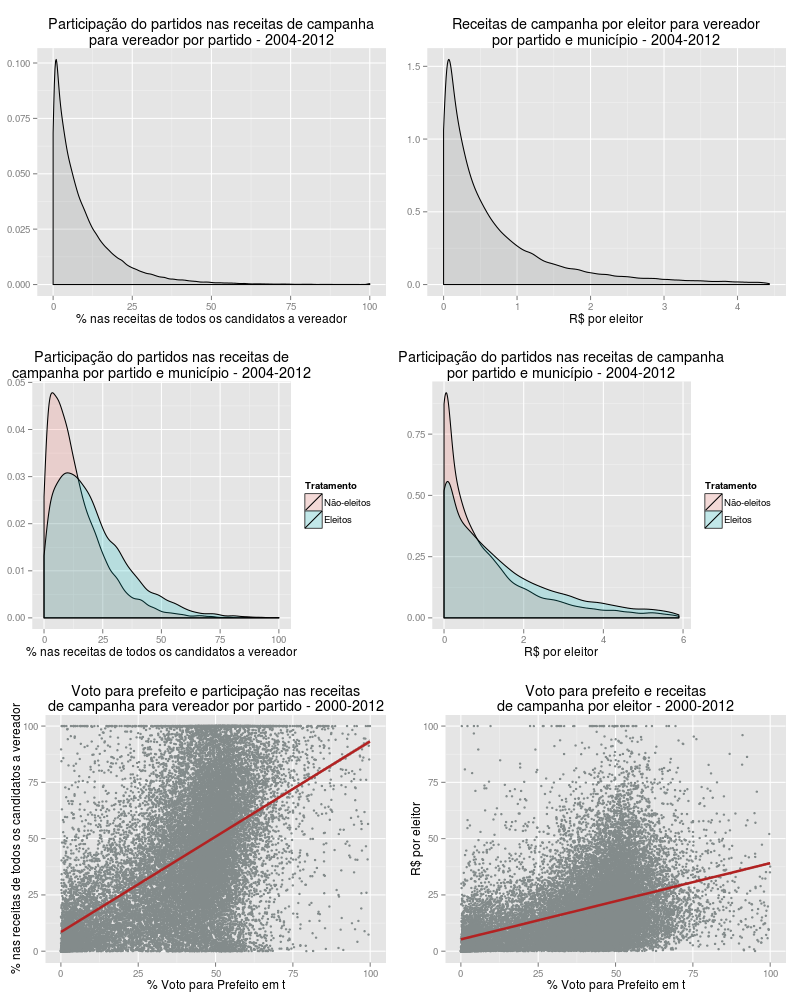
\includegraphics[scale=0.5]{c3vere1.png}
	\caption{Distribuição das receitas de campanha para vereador dos partidos (em R\$ por eleitor ou como razão do total que todos os partidos arrecadam) de 2000 a 2012: 1 - para todos os partidos em todos os municípios; 2 - para os partidos incluídos na análise e separado por grupos de tratamento; e 3 - por voto para prefeito na eleição anterior.}
	\label{fig:c3vere1}
\end{figure}


O primeiro gráfico da Figura~\ref{fig:c3vere1} apresenta a distribuição da participação do partido no total arrecadado para todos partidos os competidores na eleição para o Legislativo municipal. É bastante raro, por exemplo, que um partido arrecade mais de um quarto do total de partidos em uma determinada localidade. Esta variável tem distribuição bastante assimétrica. Em contraste, quando analisamos os gráficos que contém as observações incluídas na análise que são, por construção, os partidos mais competitivos em cada município, vemos que estes tendem a arrecadar mais do que o total da partidos no país. É possível notar que há mais casos para os valores baixos de $Y_{i}$ para partidos que perderam as eleições municipais e mais casos com valores altos de $Y_{i}$ para partidos vencedores.

A distribuição de $Y_{i}$ medida como receita por eleitor tem um comportamento praticamente idêntico ao da participação dos partidos no total de receitas em uma campanha, inclusive quanto às diferenças entre os grupos de tratamento. A grande maioria dos partidos gasta menos de R\$ 2,00 por eleitor. Também neste caso os partidos incluídos na análise têm maior dispersão, ou seja, arrecadam mais por eleitor para suas campanhas em geral mais do que a média do país.

Há uma clara correlação entre o desempenho do partido nas eleições para prefeito e as receitas dos vereadores do partido no futuro, como é possível observar nos dois últimos gráficos da Figura~\ref{fig:c3vere1}. Se no primeiro capítulo havíamos visto que o voto para vereador e prefeito em uma mesma eleição estavam correlacionados, bem como o voto para prefeito entre eleições, não causa surpresa que ambas medidas $Y_{i}$, em qualquer dos casos, estejam correlacionadas com a margem de vitória.

Para testar a validade do desenho de regressão descontínua adotado, testo o efeito do tratamento em variáveis contemporâneas à sua atribuição, novamente denominadas $O_{i}$, sendo elas as duas medidas de $Y_{i}$ para o próprio ano da eleição municipal. A Figura~\ref{fig:c3vere2} apresenta os testes:

\begin{figure}[htp]
	\centering
	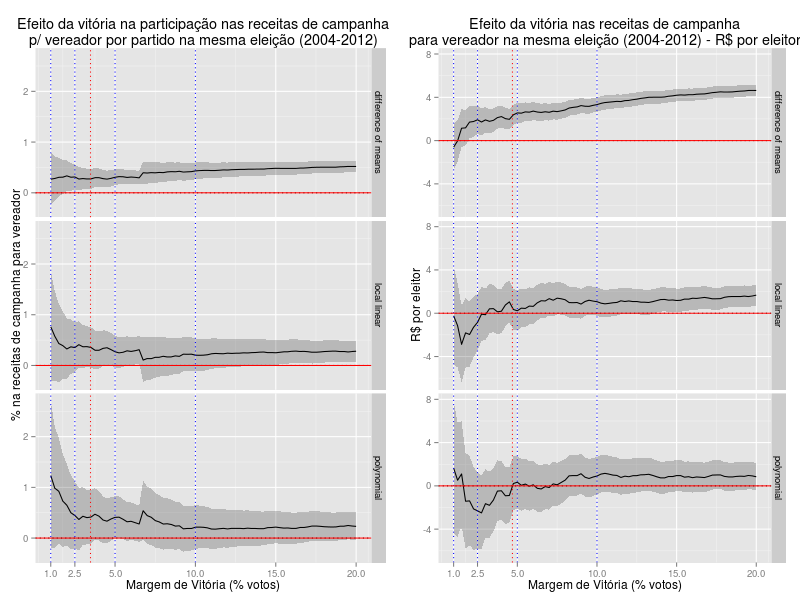
\includegraphics[scale=0.45]{c3vere2.png}
	\caption{Efeito do Tratamento nas receitas de campanha para vereador (R\$ por eleitor ou como razão do total que todos os partidos arrecadam) na mesma eleição e por margem de vitórias nas eleições para prefeito (2004-2008).}
	\label{fig:c3vere2}
\end{figure}

Diferentemente do que se observou até agora, esta seção tem um problema de validação bastante mais sério. Mais ainda, o fato de qualquer teste de validação do desenho de pesquisa adotado ser problemático compromete os resultados do desenho dos demais problemas investigados.

Quando medimos $O_{i}$ como receitas de campanha do partido para vereador por eleitor no município, os grupos de tratamento são bastante semelhantes entre si. Contudo, ao medir $O_{i}$ como proporção da receita do partido nas receitas de todos os partidos em uma localidade, vemos que, mesmo para a estimação do efeito do tratamento como descontinuidade em uma função linear ou em uma função polinomial há efeitos positivos. Para margens de vitória iguais ou menores a valores no intevalo no entre $2,5\% \leq \Delta \leq 5\%$, partidos vitoriosos arrecadaram em média cerca 0,3\% ou 0,4\% a mais do que os partidos que perderam. Se a diferença de arrecadação é um fator crucial para vencer as eleições, então não podemos afirmar que o tratamento tem comportamento \textit{quasi} aleatório quando $\tau_{i}=+\Delta$ ou $\tau_{i}=-\Delta$ e $\Delta$ tende a zero.

Uma vez que este problema é bastante sério e afeta os resultados já apresentados nos capítulos e seções anteriores, trato com mais cuidado deste tema próximo capítulo e discuto suas consequências com mais detalhes. A seguir, vamos observar os resultados do efeito do tratamento nas receitas de campanha do partido para vereador, ignorando, por ora, o problema apresentado.

\subsection{O efeito da vitória eleitoral nas receitas de campanha do partido para vereador}

Vencer as eleições para prefeito contribui para que o partido tenham mais recursos para suas campanhas futuras? Ou ainda, governar o município faz com que o partido seja capaz de atrair mais doadores de campanha? É bastante provável que políticos eleitos para prefeituras tenham mais recursos para suas campanhas próprias no futuro \footnote{O impacto de vencer as eleições nas receitas do partido para campanhas para prefeito é examinado no Capítulo\ref{cap:finaciamento}}. Mas será que a vitória no município contribui para que os membros do partido que concorrem a outros cargos consigam arrecadar mais?

Na Figura~\ref{fig:c3vere3} apresento o efeito da vitória sobre as duas medidas de $Y_{i}$ adotadas na seção, ou seja, nas receitas do partido por eleitor nas eleições para vereador seguintes e na proproção de receitas de campanha do partido dentre todas as candidaturas a vereador no município.

\begin{figure}[htp]
	\centering
	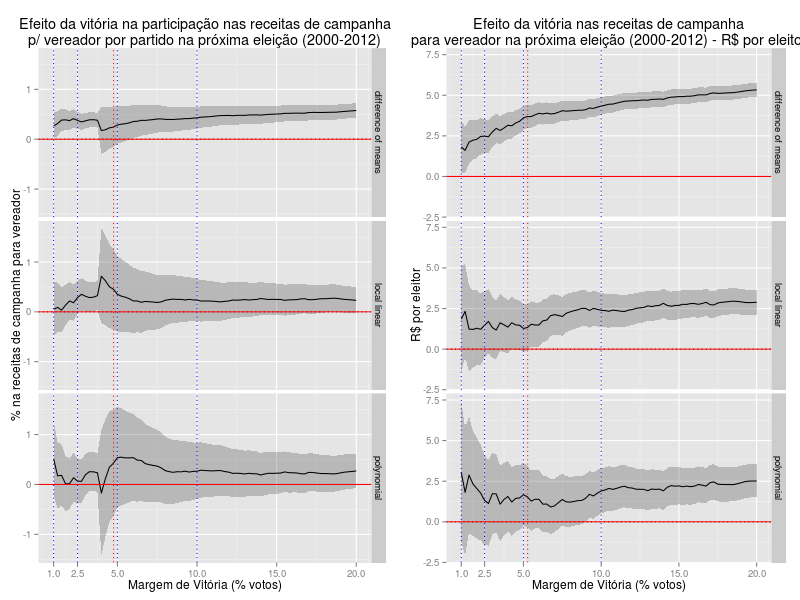
\includegraphics[scale=0.45]{c3vere3.png}
	\caption{Efeito do Tratamento nas receitas de campanha para vereador (R\$ por eleitor ou como razão do total que todos os partidos arrecadam) na eleição seguinte e por margem de vitórias nas eleições para prefeito (2000-2012).}
	\label{fig:c3vere3}
\end{figure}

Seria possível argumentar que para algumas margens de vitória específicas (no intevalo no entre $2,5\% \leq \Delta \leq 5\%$) há efeitos positivos. Em alguns pontos este efeito é diferente de zero para um intervalo de confiança de 95\% ou, em outros pontos, de 90\%, e em geral é próximo a R\$ 0,50 por eleitor. Substantivamente este valor não é irrelevante, uma vez que este valor poderia ser gasto, por exemplo, envio de material de campanha, mensagens telefônicas ou outras estratégias baratas de comunicação com os eleitores. 

Contudo, e apesar de ter termos observado diferenças importantes na distribuição das duas medidas de $Y_{i}$ para os grupos de tratamento, o resultado geral para qualquer medida ou forma de estimar é praticamente nulo. Contrariando a expectativa desta tese, portanto, concluo que o fato do partido vencer as eleições municipais ou governar a prefeitura não contribui para que os vereadores do partido consigam mais recursos para suas campanhas em comparação com as situações em que o partido não venceu a disputa pelo Executivo municipal. Ao revisar os resultados desta seção no próximo capítulo, fica a ausência de resultados fica ainda mais clara.

\section{Prefeitos, eleições municipais e alianças políticas: o efeito da vitória nas eleições para prefeito sobre o tamanho das coalizões municipais}

O último problema investigado nesta tese trata de um questão peculiar de sistemas multi-partidários. Em eleições majoritárias, como as eleições para prefeito, poucos partidos são efetivamente competitivos. De fato, como vimos no Capítulo~\ref{cap:eleicoes}, os primeiros e segundos colocados nas eleições municipais pertencem a apenas 8 partidos dentre as três dezenas de organizações oficialmente registradas e habilitadas a competir. Mesmo os oito partidos mais frequentes no topo das disputas municipais não competem recorrentemente entre si e é possível encontrar coalizões eleitorais das mais variadas no país dentro dos municípios.

A existência de eleições diretas para todos os cargos Executivos, da presidência às chefias dos estados e municípios, em combinação com a presença muitos partidos capazes de obter assentos nos Legislativos produz a necessidade de formação de coalizões de governo. Diversos trabalhos brasileiros apontam para a importância da construção de coalizões e para a os instrumentos institucionais à disposição dos chefes do Executivo em diferentes níveis de governo, que contribuem para a estabilidade das relações entre Executivo e Legislativo. Ainda que a relação entre prefeitos, vereadores e lideranças locais seja pouco investigada no Brasil, evidências empíricas apontam para a capacidade do prefeito construir coalizões e obter o apoio legislativo de vereadores. Em particular, as regras de eleboração do orçamento, aplicáveis a todo o país cujos fundamentos são constitucionais ou estão definidos em legislação federal, são centrais para a definição desta estabilidade, tal como discutivo com detalhes no capítulo anterior.

A suspeita da qual parto é que nos municípios, vereadores e membros de partidos pouco competitivos ou derrotados teriam incentivos fortes para aderirem à aliança com o partido do prefeito, fenômeno por vezes compreendido como governismo, quando este tivesse um candidato na disputa municipal. Assim, o objetivo desta seção é bastante claro: observar se partidos vitoriosos atraem apoio de outros partidos para suas candidaturas futuras, traduzido na forma de coligações eleitorais. A expectativa é que partidos vitoriosos sejam capazes de construir coligações eleitorais maiores para prefeito.

Dessa forma, utilizando novamente um desenho de regressão descontínua, observo se as coligação eleitorais para prefeitos -- medidas tanto como número de partidos na coligação, quanto como participação dos partidos da coligação nas Câmaras de Vereadores -- são maiores para os casos em que o partido venceu as eleições municipais em comparação com os casos nos quais o partido perdeu as eleições municipais. Uma possível maneira de ler o problema é: os partidos que não pretendem competir nas eleições para prefeito tendem a se aliar ao partido no governo municipal? Se sim, então devemos observar efeito do tratamento -- vencer as eleições -- no tamanho das coalizões para prefeito.

O problema investigado nesta seção está um pouco mais distante dos demais estudados até então. A base de filiados do partido ou a capacidade do partido arrecadar recursos com doadores locais estão supostamente relacionadas ao desempenho do partido nas eleições proporcionais para deputado federal, estadual e senador, por exemplo. Entretanto, conquistar apoio dos partidos locais não necessariamente se converte em um benefício para os membros do partido nos demais níveis de governo. Coalizões e coligações municipais são um assunto estritamente local, ainda que revelem um dos possíveis mecanismos para que o partido construa vantagens eleitorais no município. O interesse neste problema reside na possibilidade de existência de fenômenos análogos em outros níveis de governo, sobretudo nos estados. Governadores vencedores atraem apoio dos legisladores estaduais e dos diretórios estaduais de outros partidos? Ou ainda, como os distritos eleitorais para deputado federal e senador são os estados, será que governadores vitoriosos atraem para mais deputados federais aliados? O debate sobre o quão capazes os interesses estaduais se fazem representar no Congresso Nacional está, em alguma medida, em paralelo ao problema estudado nesta seção. Infelizmente não há eleições estaduais suficientes para repetir a pesquisa desta tese usando as eleições estuais como descontiuidade.

A seguir, explico a operacionalização da pesquisa, descrevo empiricamente as variáveis utilizadas e discuto a validade da adoção deste problema de pesquisa.

\subsection{Operacionalização da pesquisa, dados utilizados e validade do desenho de regressão descontínua}

Como medir o apoio eleitoral de partidos não competidores a um candidato a prefeito? Uma das medidas mais simples é contar o número de partidos na coligação eleitoral. Entretanto, os partidos têm relevância política bem diferentes e o peso eleitoral de seu apoio varia. Uma coligação formada por vários partidos pequenos apoiando um candidato de um partido grande na cabeça da chapa tem provavelmente menos capital político do que uma coligação formada por alguns partidos grandes e médios.

A alternativa encontrada na tese é observar o total de vereadores eleitos pelo partidos da coligação na disputa municipal anterior, ou seja, o capital político da coligação medido em termos de legisladores eleitos. Também seria viável utilizar os votos para vereador dos partidos da coligação na eleição para vereador no passado. Entretanto, estaria incluindo na análise partidos que tiveram votos mas não elegeram nenhum vereador e, portanto, tem poder de barganha reduzido ao longo do mandato do prefeito. A migração de vereadores ao longo do mandato não foi considerada, fator que potencialmente provoca ruídos nos resultados.

\begin{figure}[htp]
	\centering
	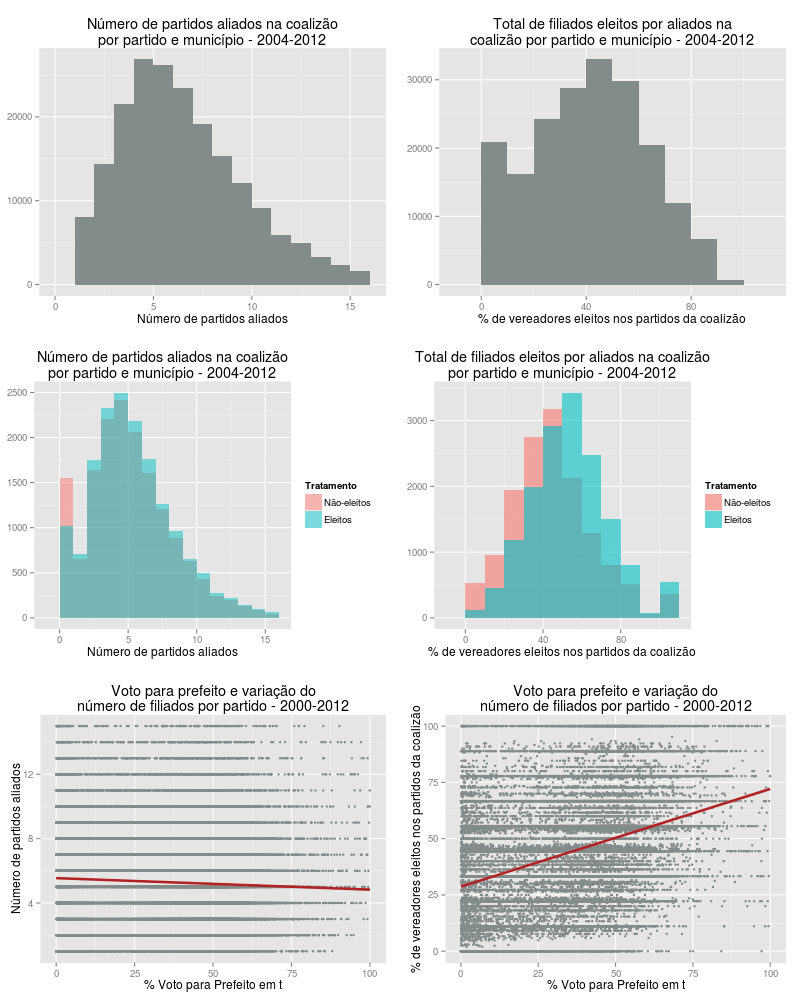
\includegraphics[scale=0.5]{c3gov1.png}
	\caption{Distribuição do tamanho das coligação municipais (em número de partidos ou como partipação dos partidos da coligação) de 2000 a 2012: 1 - para todos os partidos em todos os municípios; 2 - para os partidos incluídos na análise e separado por grupos de tratamento; e 3 - por voto para prefeito na eleição anterior.}
	\label{fig:c3gov1}
\end{figure}

O objetivo da seção é estimar o efeito do tratamento no tamanho das coalizões eleitorais do partido, $Y_{i}$ medido das duas formas apresentadas - número de partidos na coalizão eleitoral e percentual de cadeiras no Legislativo local que os partidos da coalizão conquistaram na última eleição municipal. Em ambas as medidas o partido $p$, do qual o candidato pela coalizão pertence, está sempre excluído. A Figura~\ref{fig:c3gov1} descreve as duas medidas e apresenta sua relação com a margem de vitória para prefeito. Os dois primeiros gráficos representam a distribuição para o universo; os gráficos na metade da figura repetem o procedimento, mas apenas para os dados incluídos na análise e separando por grupos de tratamento. Os últimos dois gráficos retratam a relação de $Y_{i}$ com o voto do partido para prefeito em $t$.

Muitos partidos concorrem sozinhos nas eleições municipais e há um grande número de zeros nos gráficos em que $Y_{i}$ é a contagem de partidos aliados na coalizão. Entreanto, é bastante mais comum que os partidos tenham entre 2 e 8 aliados. Há mais observações não tratadas com valor zero, ou seja, que competem em coalizões sem nenhum aliado. Para todos os demais valores, inclusive para as maiores coalizões, há sempre mais observações não tratadas.

A distribuição do tamanho das coalizões como total de vereadores eleitos pelos partidos aliados ao cabeça de chapa lembra uma curva normal, sobretudo no caso as observações que compõem a análise. Há diferenças entre os grupos de tratamento e, na média, partidos vencedores têm coalizões maiores do que partidos derrotados quando medidos $Y_{i}$ pela capacidade do partido eleger vereadores. Assim, para ambas medidas de $Y_{i}$ há suspeita de que o tratamento tenha efeito no tamanho da coalizão municipal.

A relação de cada uma das medidas com o voto para prefeito, porém, são diferentes. Aparentemente não há relação entre o voto para prefeito e o número de partidos na coligação (ou, pode-se dizer, há uma relação negativa e correlação baixa). Entretanto, a corelação entre voto para prefeito e tamanho da coalizão como número de vereadores eleitos pelos partidos aliados anteriormente é claramente positiva.

\begin{figure}[htp]
	\centering
	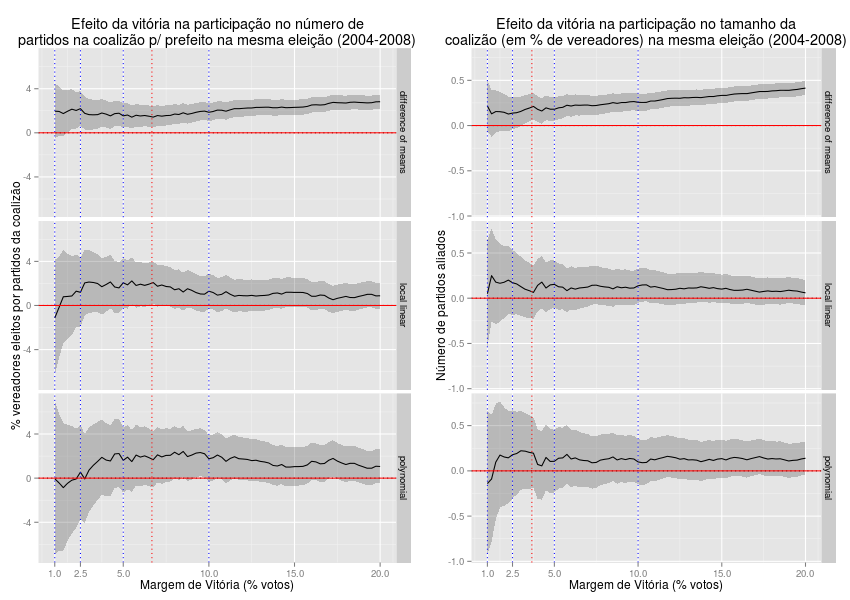
\includegraphics[scale=0.5]{c3gov2.png}
	\caption{Efeito do Tratamento no tamanho das coligação municipais (em número de partidos ou como partipação dos partidos da coligação) na mesma eleição e por margem de vitórias nas eleições para prefeito (2004-2008).}
	\label{fig:c3gov2}
\end{figure}

Seguindo padrão adotado na tese, convém testar a validade da adoção de um desenho de regressão descontínua para o problema desta seção. Novamente, $O_{i}$ representa a variável com quatro anos defasagem para qualquer uma das medidas, ou seja, para o tamanho da coalizão na própria eleição em $t$. A Figura~\ref{fig:c3gov2} apresenta o efeito do tratamento sobre $O_{i}$ estimado pelos três métodos usados no capítulo. 

Não há evidências de que o tratamento tenha algum efeito no tamanho da coalizão quando o efeito é estimado como descontinuidade em uma função, linear ou polinomial. O equilíbrio entre os grupos de tratamento aparece, porém, na estimativa por diferença de médias e, novamente, os resultados obtidos do impacto do tratamento sobre $Y_{i}$ medido desta forma não são confiáveis.

\subsection{O efeito da vitória nas eleições para prefeito sobre o tamanho das coalizões municipais}

Governar um município impacta no tamanho das coalizões do partido nas eleições para prefeito? Em outras palavras, é possível afimar que os partido que não tem pretensões de vencer as eleições tendam a se aliar com o partido que governa o município na próxima disputa municipal? Na Figura~\ref{fig:c3gov3} são apresentados os efeitos estimados do tratamento para as duas medidas - número de partidos na coalizão e total de vereadores eleitos pelos partidos da coalizão:

\begin{figure}
	\centering
	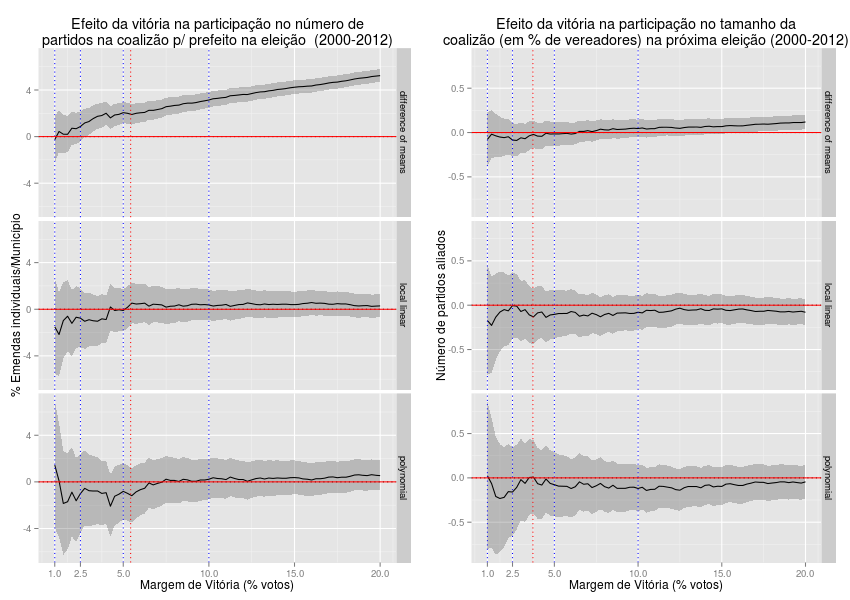
\includegraphics[scale=0.5]{c3gov3.png}
	\caption{Efeito do Tratamento no tamanho das coligação municipais (em número de partidos ou como partipação dos partidos da coligação) na eleição seguinte e por margem de vitórias nas eleições para prefeito (2000-2012).}
	\label{fig:c3gov3}
\end{figure}

Havíamos botado anteriormente que há diferenças na distribuição de $Y_{i}$ para os grupos de tratamento e a expectativa era de um efeito positivo no tamanho das coalizões. Entretanto, observamos claramente que não há efeito algum de vencer as eleições em nenhuma das duas medidas de $Y_{i}$ e para nenhuma das formas de estimação. Mais ainda, o valor estimado de $\rho$, além de não ser estatisticamente diferente de zero, é na maior parte das vezes negativo. A única excessão é a estimação por diferença de médias do efeito do tratamento no número de partidos na coaĺizão, que, como vimos, tem pouca validade.

Os resultados desta seção, como praticamente todos os resultados do capítulo, contraria a expectativa inicial. Não há evidências de que vencer as eleições tenha efeito no tamanho das coalizões eleitorais, ou seja, partidos no governo não necessariamente atraem mais aliados de outros partidos. Se nas demais seções encontramos evidências frágeis de que o tratamento tem algum efeito positivo na capacidade do partido em atrair novos membros ou doadores de campanha, quando observamos seu efeito sobre o tamanho das coligações eleitorais futuras do partido encontramos apenas resultados nulos.

\section{Breve conclusão: partidos, filiados, campanhas e efeitos nulos}

O principal objetivo deste capítulo foi explorar alguns dos possíveis mecanismos que operam, por exemplo, nos fenômenos estudados na primeira etapa da tese. Se prefeitos são capazes de afetar positivamente a performance eleitoral de candidatos de seu partido ao Câmara dos Deputados e às Assembléias Legislativas, então a investigação dos mecanismos deve ser parte da agenda de pesquisas interessadas em compreender os partidos políticos brasileiros.

A suspeita original do capítulo era de que partidos vitoriosos no município seriam capazes de atrair mais apoios políticos locais. Estes novos apoios seriam traduzidos como aumento no número de filiados, mais doadores de campanha e mais partidos nas coligações eleitorais. Entretanto, como vimos, os efeitos do tratamento em qualquer umas dessas variáveis são praticamente nulos. Portanto, não é através da conquista de novos apoios que partidos vitoriosos constroem vantagens eleitorais e outros mecanismos devem ser investigados.